\documentclass[a4paper, 12pt]{article}

\usepackage{amsmath} %Todos los paquetes de matematicas
\usepackage{amsthm}
\usepackage{mathtools}
\providecommand{\abs}[1]{\lvert#1\rvert}
\providecommand{\norm}[1]{\lVert#1\rVert}
\usepackage{yhmath}
\usepackage[utf8]{inputenc}
\usepackage[spanish]{babel}
\usepackage{wrapfig} %Figuras flotantes
\usepackage{parselines}
\usepackage{enumitem}
\usepackage{xcolor}
\usepackage{graphicx}
\graphicspath{{images/}}
\usepackage{subcaption}
\usepackage[left=2cm,right=2cm,top=2cm,bottom=2cm]{geometry}
\usepackage{eurosym} %Euro, de nada misniños

\theoremstyle{definition}
\newtheorem{ej}{Ejercicio}



\title{\textbf{Relación de ejercicios 2 EDIP}}
\author{Carlos García, Bora Goker, Javier Gómez,  \\ Ana Graciani, J.Alberto Hoces}
\date{2020/2021}

\setlength{\parindent}{0px}

\begin{document}

\maketitle

\begin{ej}
Se han estudiado 24 domicilios, obteniendo los resultados que se presentan en la siguiente tabla donde \(X\) designa el número de mascotas e \(Y\) el número de paseos a sus mascotas realizados por los dueños al día:

\begin{center}
\begin{tabular}{|c|c|c|c|c|c|c|c|c|c|c|c|c|c|c|c|c|c|c|c|c|c|c|c|c|}
\(X\) & 1 & 2 & 2 & 3 & 5 & 4 & 1 & 3 & 3 & 4 & 1 & 2 & 5 & 4 & 3 & 4 & 4 & 5 & 3 & 1 & 6 & 5 & 4 & 6 \\
\hline
\(Y\) & 2 & 3 & 1 & 4 & 3 & 2 & 6 & 4 & 1 & 6 & 6 & 5 & 1 & 2 & 5 & 1 & 1 & 2 & 6 & 6 & 2 & 1 & 2 & 5
\end{tabular}
\end{center}

Es necesario mencionar que este ejercicio carece absolutamente de interés estadístico pues no tiene ningún sentido el estudiar de manera estadística un dado que se supone totalmente aleatorio. Un enunciado más adecuado sería aquel en el que la variable \(X\) fuese el número de mascotas por hogar y la variable \(Y\) el número de paseos que se da a estas mascotas al día.

\begin{center}
    \fbox{
    \begin{minipage}[h!]{1\linewidth}
    \begin{itemize}
        \item Población: domicilios con mascotas.
        \item Tamaño de la población: 24 domicilios.
        \item Variable estadística: en este caso se presentan 2. \(X\) que es el número de mascotas por hogar e \(Y\) que es el número de paseos que se da a estas mascotas al día.
        \item Modalidades: En este caso \(X\) presenta 6 modalidades distintas al igual que \(Y\).
    \end{itemize}
    \end{minipage}
    }
\end{center}

\begin{enumerate}[label=\alph*)]
	\item Construir la tabla de frecuencias.
	
	\begin{center}
	\begin{tabular}{c|c c c c c c|c c c}
	\(X/Y\) & 1 & 2 & 3 & 4 & 5 & 6 & \(n_{i.}\) & \(n_{i.} x_i\) & \(n_{i.}x_i^2\) \\
	\hline
	1 & 0 & 1 & 0 & 0 & 0 & 4 & 4 & 4 & 4 \\
	2 & 1 & 0 & 1 & 0 & 1 & 0 & 3 & 6 & 12 \\
	3 & 1 & 0 & 0 & 2 & 1 & 1 & 5 & 15 & 45\\
	4 & 2 & 3 & 0 & 0 & 0 & 1 & 6 & 24 & 96 \\
	5 & 2 & 1 & 1 & 0 & 0 & 0 & 4 & 20 & 100 \\
	6 & 0 & 1 & 0 & 0 & 1 & 0 & 2 & 12 & 72\\
	\hline 
	\(n_{.j}\) & 6 & 6 & 2 & 2 & 3 & 5 & 24 & 81 & 329 \\
	\(n_{.j} y_j\) & 6 & 12 & 6 & 8 & 15 & 30 & 77 & & \\
	\(n_{.j}y_j^2\) & 6 & 24 & 18 & 32 & 75 & 180 & 335 & & \\
	\end{tabular}
	\end{center}
	
	\item Calcular las medias de mascotas y paseos por domicilio y ver cuales son más homogéneas.
	
	Primero calcularemos lo pedido para la variable \(X\):
	
\[
	\overline{x} = \frac{1}{n} \sum_{i=1}^{k} n_{i.}x_i = \frac{81}{24} = 3.375 \text{ mascotas}
\]
\[
	\sigma_x^2 = \frac{1}{n} \sum_{i=1}^{k} n_{i.} (x_i - \overline{x})^2 = \frac{329}{24} - \left(\frac{81}{24}\right)^2 = 2.317 \text{ mascotas}^2
\]
\[
	C.V.(x) = \frac{\sigma_x}{\abs{\overline{x}}} = \frac{\sqrt{2.317}}{3.375} = 0.451
\]

Ahora pasamos a la variable \(Y\):
\[
	\overline{y} = \frac{1}{n} \sum_{j=1}^{p} n_{.j} y_j = \frac{77}{24} = 3.208 \text{ paseos}
\]
\[
	\sigma_y^2 = \frac{1}{n} \sum_{j=1}^{p} n_{.j}(y_j - \overline{y})^2 = \frac{335}{24} - \left( \frac{77}{24} \right)^2 = 3.664 \text{ paseos}^2
\]
\[
	C.V.(y) = \frac{\sigma_y}{\abs{\overline{y}}} = \frac{\sqrt{3.664}}{3.208} = 0.596
\]

Podemos observar que la primera distribución presenta un coeficiente de variación menor que la segunda y por tanto podemos afirmar que esta es la más homogénea de las dos.

	\item ¿Qué resultado del segundo dado es más frecuente cuando en el primero se obtiene un 3?
	
	Podemos observar que:
\[
	n_{34} > n_{3j} \quad \forall j \in \{1,2,3,5,6\}
\]
De entre los domicilios con 3 mascotas, el resultado más frecuente es 4 paseos.

	\item Calcular las mascotas máximas del 50\% de las puntuaciones de los domicilios en los que se han hecho 2 o 5 paseos.
	
\begin{center}
\begin{tabular}{|c|c|c|}
	\hline
	\(x_i\) & \(n_{i2} + n_{i5}\) & \(N_{i2} + N_{i5}\) \\
	\hline
	1 & 1 & 1 \\
	2 & 1 & 2 \\
	3 & 1 & 3 \\
	4 & 3 & 6 \\
	5 & 1 & 7 \\
	6 & 2 & 9 \\
	\hline
\end{tabular}
\end{center}

\[
	\frac{50}{100} \cdot 9 = 4.5 \Rightarrow Me = 4 \text{ mascotas}
\]
\end{enumerate}
\end{ej}

\begin{ej}
Medidos los pesos, X (en Kg), y las alturas, Y (en cm), a un grupo de individuos, se han obtenido
los siguientes resultados:

\begin{center}
\begin{tabular}{c|cccccc}
	\(X/Y\) & 160 & 162 & 164 & 166 & 168 & 170 \\
	\hline
	48 & 3 & 2 & 2 & 1 & 0 & 0 \\
	51 & 2 & 3 & 4 & 2 & 2 & 1 \\
	54 & 1 & 3 & 6 & 8 & 5 & 1 \\
	57 & 0 & 0 & 1 & 2 & 8 & 3 \\
	60 & 0 & 0 & 0 & 2 & 4 & 4\\
\end{tabular}
\end{center}

\begin{center}
    \fbox{
    \begin{minipage}[h!]{1\linewidth}
    \begin{itemize}
        \item Población: grupo de individuos.
        \item Tamaño de la población: 70 individuos.
        \item Variable estadística: en este caso se presentan 2. \(X\) que es el peso del individuo e \(Y\) que es la altura del mismo.
    \end{itemize}
    \end{minipage}
    }
\end{center}

\begin{enumerate}[label=\alph*)]
	\item Calcular el peso medio y la altura media y decir cuál es más representativo.
	
	Para ello hemos de trabajar con las distribuciones marginales del carácter X (peso en Kg) y del carácter Y (altura en cm). Tras efectuar los cálculos pertinentes, la tabla anterior queda de la siguiente forma:
	
	\begin{center}
\begin{tabular}{c|cccccc|ccc}
	\(X/Y\) & 160 & 162 & 164 & 166 & 168 & 170 & \(n_{i.}\) & \(n_{i.}x_i\) & \(n_{i.}x_i^2\) \\
	\hline
	48 & 3 & 2 & 2 & 1 & 0 & 0 & 8 & 384 & 18432 \\
	51 & 2 & 3 & 4 & 2 & 2 & 1 & 14 & 714 & 36414\\
	54 & 1 & 3 & 6 & 8 & 5 & 1 & 24 & 1296 & 69984\\
	57 & 0 & 0 & 1 & 2 & 8 & 3 & 14 & 798 & 45486\\
	60 & 0 & 0 & 0 & 2 & 4 & 4 & 10 & 600 & 36000\\
	\hline
	\(n_{.j}\) & 6 & 8 & 13 & 15 & 19 & 9\\
	\(n_{.j} y_j\) & 960 & 1296 & 2132 & 2490 & 3192 & 1530\\
	\(n_{.j} y_j^2\) & 153600 & 209952 & 349648 & 413340 & 536256 & 260100\\
\end{tabular}
\end{center}

\[
	\bar{x} = \frac{1}{n} \sum_{i=1}^{5} x_i n_{i.} = \frac{384+714+1296+798+600}{70} = 54.1714 \text{ kilogramos} 
\]

\[
	\bar{y} = \frac{1}{n} \sum_{j=1}^{6} y_j n_{.j} = \frac{960+1296+2132+2490+3192+1530}{70} = 165.7143 \text{ centímetros} 
\]

Para poder determinar cuál de las dos medias es más representativa, haremos uso del coeficiente de variación de Pearson, el cual nos permitirá interpretar independientemente de la escala la variabilidad de los datos respecto de su media:

\[
	\sigma_x = \sqrt{\frac{1}{n} \sum_{i=1}^{5} n_{i.} x_i^2 - \overline{x}^2} = 3.582 \text{ kilogramos} \qquad C.V(X) = \frac{\sigma_x}{\bar{x}} = 0.0661
\]

\[
	\sigma_y = \sqrt{\frac{1}{n} \sum_{j=1}^{6} n_{.j} y_j^2 - \overline{y}^2} = 2.9519 \text{ centímetros} \qquad C.V(Y) = \frac{\sigma_y}{\bar{y}} = 0.0178
\]

En vista de los resultados, se deduce que la distribución marginal del carácter Y (la altura en cm) es más homogénea, por lo que la altura media es la más representativa de las dos.

 \item Calcular el porcentaje de individuos que pesan menos de 55 Kg y miden más de 165 cm.
 
Si miden más de 165 cm y pesan menos de 55 kg, hemos de tener en cuenta las frecuencias absolutas de todos los pares $(x_i,y_j)$ con $i \in \{1,2,3\}$ e $j \in \{4,5,6\}$. Efectuamos el cálculo:

\[
	100 \cdot \frac{1}{n} \cdot \sum_{j=4}^{6}\sum_{i=1}^{3}n_{ij} = 100 \cdot \frac{1}{70} \cdot (1+2+2+1+8+5+1) = 28.571\% \text{ de los individuos} 
\]

\item Entre los que miden más de 165 cm, ¿cuál es el porcentaje de los que pesan más de 52 Kg?

Si miden más de 165 cm y pesan más de 52 kg, hemos de tener en cuenta las frecuencias absolutas de todos los pares $(x_i,y_j)$ con $i \in \{3,4,5\}$ e $j \in \{4,5,6\}$. Efectuamos el cálculo:

\[
	100 \cdot \frac{1}{n} \cdot \sum_{j=4}^{6}\sum_{i=3}^{5}n_{ij} = 100 \cdot \frac{1}{70} \cdot (8+5+1+2+8+3+2+4+4) = 52.857\% \text{ de los individuos} 
\]

\item ¿Cuál es la altura más frecuente entre los individuos cuyo peso oscila entre 51 y 57 Kg?

Esto es equivalente a hallar la modalidad $y_j$ a la que le corresponde el máximo de $n_{2j}+n_{3j}+n_{4j}$:

\begin{center}
\begin{tabular}{c|c}
	\(y_j\) & \(n_{2j}+n_{3j}+n_{4j}\)\\
	\hline
	160 & 3 \\
	162 & 6\\
	164 & 11\\
	166 & 12\\
	168 & 15\\
	170 & 5\\
\end{tabular}
\end{center}

De la tabla se obtiene que la altura más frecuente entre los individuos cuyo peso oscila entre 51 y 57 kg es $y_5 = 168$ cm.

\item ¿Qué peso medio es más representativo, el de los individuos que miden 164 cm o el de los
que miden 168 cm?

Para poder determinar lo que se nos pide, hemos de estudiar de estudiar dos distribuciones condicionadas: la del carácter X condicionada a la modalidad $y_3$ y la del carácter X condicionada a la modalidad $y_5$:

\begin{center}
\begin{tabular}{c|c|c|c}
	\(x_i\) & \(n_{i3}\) & \(x_i n_{i3}\) & \(x_{i}^{2} n_{i3}\)\\
	\hline
	48 & 2 & 96 & 4608\\
	51 & 4 & 204 & 10404\\
	54 & 6 & 324 & 17496\\
	57 & 1 & 57 & 3249\\
	60 & 0 & 0 & 0\\
	\hline
	& 13 & 681 & 35757\\
\end{tabular}
\qquad
\begin{tabular}{c|c|c|c}
	\(x_i\) & \(n_{i5}\) & \(x_i n_{i5}\) & \(x_{i}^{2} n_{i5}\)\\
	\hline
	48 & 0 & 0 & 0\\
	51 & 2 & 102 & 5202\\
	54 & 5 & 270 & 14580\\
	57 & 8 & 456 & 25992\\
	60 & 4 & 240 & 14400\\
	\hline
	& 19 & 1068 & 60174\\
\end{tabular}
\end{center}

\[
	\bar{x}_{3} = \frac{1}{n} \sum_{i=1}^{5} x_i n_{i3} = \frac{681}{13} =  52.3846\text{ kg} \qquad \bar{x}_{5} = \frac{1}{n} \sum_{i=1}^{5} x_i n_{i5} = \frac{1068}{19} =  56.2105\text{ kg} 
\]

\[
	\sigma_{x,3} = \sqrt{\frac{1}{n} \sum_{i=1}^{5} n_{i3} x_i^2 - \overline{x}_{3}^{2}} = 2.5283 \text{ kg} \qquad \sigma_{x,5} = \sqrt{\frac{1}{n} \sum_{i=1}^{5} n_{i5} x_i^2 - \overline{x}_{5}^{2}} = 2.7216 \text{ kg}
\]

Al igual que se ha hecho en el apartado a), haremos uso del coeficiente de variación de Pearson para poder determinar qué peso medio es más representativo:

\[
	C.V_3(Y) = \frac{\sigma_{x,3}}{\bar{x}_{3}} = 0.0483 \qquad C.V_5(Y) = \frac{\sigma_{x,5}}{\bar{x}_{5}} = 0.0484
\]

En vista de lo obtenido, podemos concluir que el peso medio de la distribución condicionada del carácter X a la modalidad $y_3$ es el más representativo de los dos, aunque en este caso los coeficientes de Pearson son prácticamente iguales.
\end{enumerate}
\end{ej}

\begin{ej}
En una encuesta de familias sobre el número de individuos que la componen \((X)\) y el número de personas activas en ellas \((Y)\) se han obtenido los siguientes resultados:
\begin{center}
\begin{tabular}{c|cccc}
	\(X/Y\) & 1 & 2 & 3 & 4 \\
	\hline
	1 & 7 & 0 & 0 & 0 \\
	2 & 10 & 2 & 0 & 0 \\
	3 & 11 & 5 & 1 & 0 \\
	4 & 10 & 6 & 6 & 0 \\
	5 & 8 & 6 & 4 & 2 \\
	6 & 1 & 2 & 3 & 1 \\
	7 & 1 & 0 & 0 & 1 \\
	8 & 0 & 0 & 1 & 1
\end{tabular}
\end{center}

\begin{center}
    \fbox{
    \begin{minipage}[h!]{1\linewidth}
    \begin{itemize}
        \item Población: un grupo de familias.
        \item Tamaño de la población: 89 familias.
        \item Variable estadística: en este caso se presentan 2. \(X\) que es el número de individuos de cada familia e \(Y\) que es la cantidad de personas activas en las mismas.
    \end{itemize}
    \end{minipage}
    }
\end{center}

\begin{enumerate}[label=\alph*)]
	\item Calcular la recta de regresión de \(Y\) sobre \(X\).
	\begin{center}
	\begin{tabular}{c|c c c c | c c c}
	\(X/Y\) & 1 & 2 & 3 & 4 & \(n_{i.}\) & \(n_{i.}x_i\) & \(n_{i.}x_i^2\) \\
	\hline
	1 & 7 & 0 & 0 & 0 & 7 & 7 & 7 \\
	2 & 10 & 2 & 0 & 0 & 12 & 24 & 48 \\
	3 & 11 & 5 & 1 & 0 & 17 & 51 & 153 \\
	4 & 10 & 6 & 6 & 0 & 22 & 88 & 352 \\
	5 & 8 & 6 & 4 & 2 & 20 & 100 & 500 \\
	6 & 1 & 2 & 3 & 1 & 7 & 43 & 252 \\
	7 & 1 & 0 & 0 & 1 & 2 & 14 & 98 \\
	8 & 0 & 0 & 1 & 1 & 2 & 16 & 128 \\
	\hline
	\(n_{.j}\) & 48 & 21 & 15 & 5 & 89 \\
	\(n_{.j} y_j\) & 48 & 42 & 45 & 20 \\
	\(n_{.j} y_j^2\) & 48 & 84 & 135 & 80 \\
	\end{tabular}
	\end{center}
	
La recta de regresión lineal de \(Y\) sobre \(X\) viene dada por la expresión:
\[
	y - \overline{y}  =\frac{\sigma_{xy}}{\sigma_x^2} (x - \overline{x}) \Rightarrow y = \frac{\sigma_{xy}}{\sigma_x^2}x - \frac{\sigma_{xy}}{\sigma_x^2} \overline{x} + \overline{y}
\]
Por lo tanto, comencemos calculando las medias aritméticas y la varianza de \(x\) y la covarianza:
\[
	\overline{x} = \frac{1}{n} \sum_{i=1}^{8} x_i n_{i.} = 3.8427 \text{ individuos} \qquad \overline{y} = \frac{1}{n} \sum_{j=1}^{4} y_j n_{.j} = 1.7416 \text{ personas activas}
\]
\[
	\sigma_x^2 = \frac{1}{n} \sum_{i=1}^{8} n_{i.} x_i^2 - \overline{x}^2 = 2.5146 \text{ individuos}^2
\]
\[
	\sigma_{xy} = \frac{1}{n} \sum_{i=1}^{8} \sum_{j=1}^{4} n_{ij} x_i y_j - \overline{x}\ \overline{y} = 0.7907
\]
Por lo tanto, la recta de regresión de \(Y\) sobre \(X\) quedaría:
\[
	y = \frac{\sigma_{xy}}{\sigma_x^2}x - \frac{\sigma_{xy}}{\sigma_x^2} \overline{x} + \overline{y} = 0.3144x + 0.5333
\]

	\item ¿Es adecuado suponer una relación lineal para explicar el comportamiento de \(Y\) a partir de \(X\)?
	
Para ver cómo de adecuado es suponer dicha relación calculamos el coeficiente de correlación lineal:
\[
	r^2 = \sqrt{\frac{\sigma_{xy}^2}{\sigma_x^2 \sigma_y^2}} \qquad r = \sqrt{r^2}
\]
Ahora calculamos la varianza de \(Y\):
\[
	\sigma_y^2 = \frac{1}{n} \sum_{j=1}^{4} n_{.j} y_j^2 - \overline{y}^2 = 0.8657 \text{ personas activas}^2
\]
Por tanto:
\[
	r^2 = \frac{0.7907^2}{2.5146 \cdot 0.8657} = 0.2872 \qquad r = 0.536
\]
Observando estos resultados podemos afirmar que no es adecuado suponer esta relación linear puesto que el $r^2$ está demasiado alejado de 1 y el modelo explica menos del 29\% de los casos.

\begin{figure}[h!]
	\centering
temperaturas	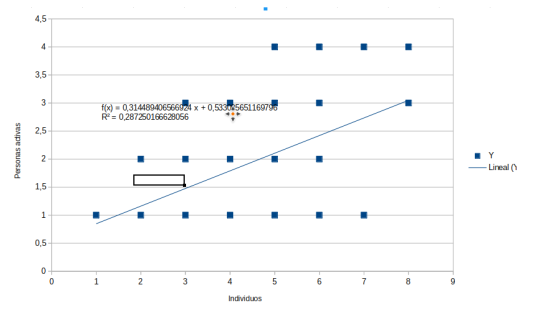
\includegraphics[scale=0.55]{images/ejer3.png}
\end{figure}

\end{enumerate}

\end{ej}

\begin{ej}
Se realiza un estudio sobre la tensión de vapor de agua ($Y$ , en ml. de Hg.) a distintas temperaturas
($X$, en ºC). Efectuadas 21 medidas, los resultados son:

\begin{center}
\begin{tabular}{c|ccc}
    $X/Y$ & $(0.5, 1.5]$ & $(1.5, 2.5]$ & $(2.5, 5.5]$ \\
    \hline
    $(1, 15]$ & 4 & 2 & 0 \\
    $(15, 25]$ & 1 & 4 & 2 \\
    $(25, 30]$ & 0 & 3 & 5 \\
\end{tabular}
\end{center}

Explicar el comportamiento de la tensión de vapor en términos de la temperatura mediante una
función lineal. ¿Es adecuado asumir este tipo de relación? \\

\begin{center}
    \fbox{
    \begin{minipage}[h!]{1\linewidth}
    \begin{itemize}
        \item Población: las distintas mediciones.
        \item Tamaño de la población: 21 mediciones.
        \item Variable estadística: en este caso se presentan 2. \(X\) que es la temperatura e \(Y\) que es la tensión del vapor de agua en \(ml\) de \(Hg\).
        \end{itemize}
    \end{minipage}
    }
\end{center}

\(n_{13} =  0 \not= \frac{6\cdot7}{21} = \frac{n_{1\cdot}\cdot n_{\cdot3}}{n}\Longrightarrow\) existe al menos un par de valores de las variables tal que la frecuencia absoluta nde ese par o coincide con el producto de las de las marginales partido por el tamaño de la población, lego podemos afirmar que $X$ e $Y$ no son independientes. \\

Buscamos la recta de regresión $Y/X$:
\[
y - \overline{y} = \frac{\sigma_{xy}}{\sigma_{x}^2} \cdot (x - \overline{x})
\]

Escribimos la tabla utilizando las marcas de clase:  \\

\begin{center}
\begin{tabular}{c|ccc|ccc}
    $X/Y$ & 1 & 2 & 4 & $n_{i.}$ & $c_i n_{i.}$ & $c_i^2 n_{i.}$ \\
    \hline
    8 & 4 & 2 & 0 & 6 & 48 & 384 \\
    20 & 1 & 4 & 2 & 7 & 140 & 2800 \\
    27,5 & 0 & 3 & 5 & 8 & 220 & 6050 \\
    \hline
    $n_{.j}$ & 5 & 9 & 7 & 21 & 408 & 9234 \\
    $d_{j}n_{.j}$ & 5 & 18 & 28 & 51 \\
    $d_{j}^2 n_{.j}$ & 5 & 36 & 112 & 153 \\
\end{tabular}
\end{center} 

Media de la distribución marginal de $X$:
\[
\overline{x} = \frac{1}{n}\cdot \sum_{i=1}^3 c_i\cdot n_{i.} = \frac{408}{21} = 19.429^{\circ}C
\]
Media de la distribución marginal de $Y$:
\[
\overline{y} = \frac{1}{n}\cdot \sum_{j=1}^3 d_j\cdot n_{.j} = \frac{51}{21} = 2.429\text{ ml. de Hg}
\]
Varianza de la marginal de $X$:
\[
\sigma_x^2 = \frac{1}{n}\cdot \sum_{i=1}^3 (n_{i.}  c_i^2) -\overline{x}^2 = \frac{9234}{21} - 19.429^2 = 62.226^{\circ} C^2
\]
Varianza de la marginal de $Y$:
\[
\sigma_y^2 = \frac{1}{n}\cdot \sum_{j=1}^3 (n_{.j}  d_j^2) -\overline{y}^2 = 1.386 \text{ ml² de Hg}
\]
Covarianza de las variables $X$ e $Y$:
\[
Cov(X,Y) = \sigma_{xy} = \frac{1}{n} \sum_{i=1}^3\sum_{j=1}^3 n_{ij} c_{i} d_{j} - \overline{x} \overline{y} = \frac{1119}{21} - 19,429\cdot 2.429 = 6.093
\]
Recta de regresión:
\[
y = ax + b = \frac{\sigma_{xy}}{\sigma_x^2}x + \overline{y} - \frac{\sigma_{xy}}{\sigma_x^2}\overline{x} \\
\]

\(
a= \frac{\sigma_{xy}}{\sigma_x^2} = \frac{6.093}{62.228}= 0.098 ; \\
b= \overline{y} - a\overline{x} = 2.429 - 0.098\cdot 19.429 = 0.525;
\)
\[
y=0.098x + 0.525
\]
Razón de correlación:
\[
\eta_{Y/X}^{2} = \eta_{X/Y}^{2} = r^2 = \frac{\sigma_{xy}^2}{\sigma_x^2 \sigma_y^2} = \frac{6.093^2}{62.228\cdot 1386} = 0.430
\]
La recta de regresión explica el 43\% de los casos, menos del 50\%, luego podemos concluir que no se trata de un buen ajuste. \\


\end{ej}


\begin{ej}
Estudiar la dependencia o independencia de las variables en cada una de las siguientes distribuciones. Dar, en cada caso las curvas de regresión y la covarianza de las dos variables. \\

\par

Comencemos con la primera distribución:

\begin{center}
\begin{tabular}{c|ccccc}
	\(X/Y\) & 1 & 2 & 3 & 4 & 5 \\
	\hline
	10 & 2 & 4 & 6 & 10 & 8 \\
	20 & 1 & 2 & 3 & 5 & 4 \\
	30 & 3 & 6 & 9 & 15 & 12 \\
	40 & 4 & 8 & 12 & 20 & 16
\end{tabular}
\end{center}

Debemos saber que el cáracter \(Y\) es independiente a nivel estadístico del carácter \(X\) si las distribuciones de \(Y\) condicionadas a cada valor de la variable \(X\) son iguales \(\forall x_i \quad i = 1, 2, \dotsc, k\):
\[
	f_j^i = f_{j/i}
\]

Así, se tiene que cumplir lo siguiente:
\begin{equation} \label{ref:independenciaXY}
	\frac{n_{1j}}{n_{1.}} = \frac{n_{2j}}{n_{2.}} = \dotsm = \frac{n_{ij}}{n_{i.}} = \dotsm = \frac{n_{kj}}{n_{k.}} \qquad \forall j = 1,2, \dotsc, p
\end{equation}

Ahora comprobemos si esto se cumple en la distribución representada por la tabla anterior. Es digno de mención que el recíproco también es cierto, es decir, si \(Y\) es independiente de \(X\), \(X\) también lo es de \(Y\).
\[
	j = 1 \qquad \frac{2}{30} = \frac{1}{15} = \frac{3}{45} = \frac{4}{60}
\]
\[
	j = 2 \qquad \frac{4}{30} = \frac{2}{15} = \frac{6}{45} = \frac{8}{60}
\]
\[
	j = 3 \qquad \frac{6}{30} = \frac{3}{15} = \frac{9}{45} = \frac{12}{60}
\]
\[
	j = 4 \qquad \frac{10}{30} = \frac{5}{15} = \frac{15}{45} = \frac{20}{60}
\]
\[
	j = 5 \qquad \frac{8}{30} = \frac{4}{15} = \frac{12}{45} = \frac{16}{60}
\]

Podemos observar que, efectivamente, \(Y\) es independiente de \(X\) y por tanto carece de sentido estudiar la curva de regresión ya que su objetivo principal es predecir el valor de la variable dependiente $Y$ dado el valor $x_i$ de la variable independiente asociada $X$, es decir, predecir el comportamiento de la variable condicionada $Y/X = x_i$, el cual ya sabemos pues $\frac{n_{1j}}{n_{1.}} = \frac{n_{2j}}{n_{2.}} = \dotsm = \frac{n_{ij}}{n_{i.}} = \dotsm = \frac{n_{kj}}{n_{k.}}$. Afirmamos que:
\[
	\sigma_{xy} = 0
\]

\par 

Ahora pasemos a estudiar la segunda distribución:
\begin{center}
\begin{tabular}{c|ccc}
	\(X/Y\) & 1 & 2 & 3 \\
	\hline
	-1 & 0 & 1 & 0 \\
	0 & 1 & 0 & 1 \\
	1 & 0 & 1 & 0
\end{tabular}
\end{center}

De entrada, podemos observar que estas dos variables no son independientes, puesto que si hubiese algún \(n_{ij} = 0\), la igualdad (\ref{ref:independenciaXY}) no se daría a no ser que \(n_{ij} = 0 \quad \forall i,j\), lo cual volvería absurdo el estudio de esta tabla puesto que no representaría ninguna distribución de frecuencias. \\

Ahora observemos la posible dependencia funcional. Podemos afirmar que \(X\) no depende funcionalmente, pues \(n_{12} = 1\) y \(n_{22} = 0\), es decir, a la modalidad 2 de \(Y\) le corresponden dos posibles modalidades de \(X\). \\

\begin{center}
\begin{tabular}{c|cccc}
	\(X/Y\) & 1 & 2 & 3 & \(n_{i.} x_i\) \\
	\hline
	-1 & 0 & 1 & 0 & -1 \\
	0 & 1 & 0 & 1 & 0 \\
	1 & 0 & 1 & 0 & 1
\end{tabular}
\end{center}

Calculemos la covarianza:
\[
	\sigma_{xy} = m_{11} - \overline{x}\ \overline{y}
\]
\[
	\overline{x} = \frac{1}{n} \sum_{i=1}^{3} n_{i.} x_i = 0
\]

Al ser \(\overline{x} = 0\), la covarianza será \(m_{11}\):
\[
	\sigma_{xy} = \sum_{i=1}^{3} \sum_{j=1}^{3} f_{ij} x_i y_j = 0
\]

Este resultado nos demuestra que si las variables son independientes, su covarianza es 0, pero el recíproco no es cierto. Aquí las variables no son independientes y su covarianza es 0. \\

Ahora calcularemos la curva de regresión de tipo 1 de \(Y/X\), que es la curva que pasa por los puntos \((x_i, \overline{y}_i) \quad i=1, \dotsc, k\). \\

Punto 1: \((-1, 2)\) \hspace{1cm} Punto 2: \((0, 2)\) \hspace{1cm} Punto 3: \((1, 2)\)

\begin{figure}[!h]
	\centering
	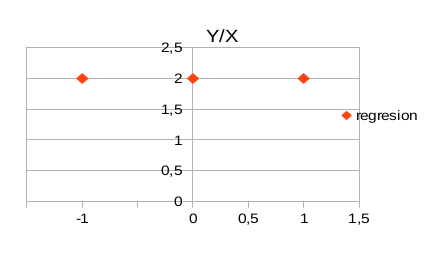
\includegraphics[scale=0.6]{images/ejer5_Y_X.png}
\end{figure}

\par 

Ahora calcularemos la curva de regresión tipo 1 de \(X/Y\), la cual pasa por los puntos \(\overline{x}_j, y_j \quad j = 1, \dotsc, p\). \\

Punto 1: \((0, 1)\) \hspace{1cm} Punto 2: \((0, 2)\) \hspace{1cm} Punto 3: \((0, 3)\)

\begin{figure}[!h]
	\centering
	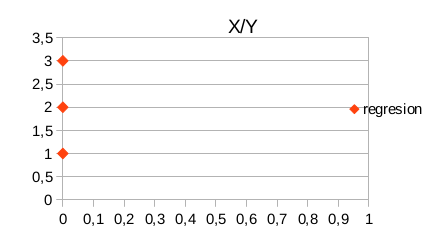
\includegraphics[scale=0.6]{images/ejer_5_X_Y.png}
\end{figure}

\end{ej}

\begin{ej}
Dada la siguiente distribución bidemensional:

\begin{center}
\begin{tabular}{c | c c c c}
	\(X/Y\) & 1 & 2 & 3 & 4 \\
	\hline
	10 & 1 & 3 & 0 & 0 \\
	12 & 0 & 1 & 4 & 3 \\
	14 & 2 & 0 & 0 & 2 \\
	16 & 4 & 0 & 0 & 0
\end{tabular}
\end{center}

Ampliamos la tabla calculando datos que nos resultarán de utilidad

\begin{center}
	\begin{tabular}{c | c c c c | c c c c}
	\(X/Y\) & 1 & 2 & 3 & 4 & \(n_{i.}\) & \(n_{i.} x_i\) & \(n_{i.} x_i^2\) & $\overline{y}_i$\\
	\hline
	10 & 1 & 3 & 0 & 0 & 4 & 40 & 400 & 1,75\\
	12 & 0 & 1 & 4 & 3 & 8 & 96 & 1152 & 3,25\\
	14 & 2 & 0 & 0 & 2 & 4 & 56 & 784 & 2,5\\
	16 & 4 & 0 & 0 & 0 & 4 & 64 & 1024 & 1\\
	\hline
	\(n_{.j}\) & 7 & 4 & 4 & 5 & 20 & 256 & 3360 & \\
	\(n_{.j} y_j\) & 7 & 8 & 12 & 20 & 47 \\
	\(n_{.j} y_j^2\) & 7 & 16 & 36 & 80 & 139 \\
	$\overline{x}_j$ & 14,571 & 10,5 & 12 & 12,8
	\end{tabular}
	\end{center}
\begin{enumerate}[label=\alph*)]
	\item ¿Son estadísticamente independientes \(X\) e \(Y\)?
	
	\(n_{13} =  0 \not= \frac{4\cdot4}{20} = \frac{n_{1\cdot}\cdot n_{\cdot3}}{n}\Longrightarrow\) existe al menos un par de valores de las variables tal que la frecuencia absoluta nde ese par o coincide con el producto de las de las marginales partido por el tamaño de la población, lego podemos afirmar que $X$ e $Y$ no son independientes.\\ También observamos que como para cada modalidad de \(X\) no encontramos una única modalidad de \(Y\) con frecuencia no nula y por tanto tampoco son funcionalmente dependientes.
	
	
	\item Calcular y representar las curvas de regresión de \(X/Y\) e \(Y/X\).
	
	Para calcular la curva de regresión de tipo I de \(X/Y\) tenemos que calcular los puntos por los que pasa. Estos son los puntos \((\overline{x}_j, y_j) \quad j=1,\dotsc, p.\)
\[
	\overline{x}_1 = \frac{10 + 14 \cdot 2 + 16 \cdot4}{7} = 14.57 \qquad \overline{x}_2 = \frac{10 \cdot 3 + 12}{4} = 10.5
\]
\[
	\overline{x}_3 = \frac{12 \cdot 4}{4} = 12 \qquad \overline{x}_4 = \frac{12 \cdot 3 + 14 \cdot 2}{5} = 12.8
\]

Puntos:\qquad(14.57, 1)\qquad(10.5, 2)\qquad\((12, 3)\)\qquad(12.8, 4)


\begin{figure}[h!]
\centering
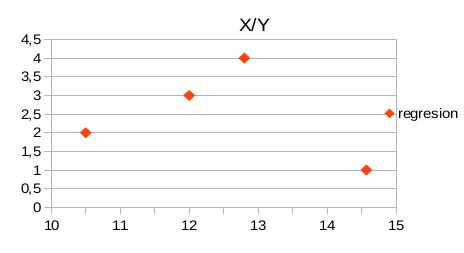
\includegraphics[scale=0.5]{images/ejer_6_X_Y.png}
\end{figure}

Ahora calculamos la curva de regresión de tipo I de \(Y/X\), la cual pasa por los puntos \((x_i, \overline{y}_i) \quad i=1,\dotsc,k\)
\[
	\overline{y}_{1} = \frac{1 + 2 \cdot 3}{4} = 1.75 \qquad \overline{y}_{2} = \frac{2 + 3 \cdot 4 + 4 \cdot 3}{8} = 3.25
\]
\[
	\overline{y}_{3} = \frac{2 + 2 \cdot 4}{4} = 2.5 \qquad \overline{y}_{4} = \frac{4}{4} = 1
\]

Puntos:\qquad(10, 1.75)\qquad(12, 3.25)\qquad(14, 2.5)\qquad(16, 1)

\begin{figure}[h!]
\centering
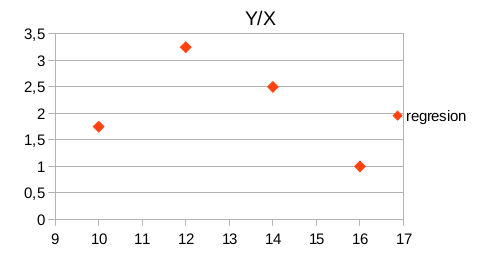
\includegraphics[scale=0.5]{images/ejer_6_Y_X.png}
\end{figure}

	\item Cuantificar el grado en que cada variable es explicada por la otra mediante la correspondiente curva de regresión. \\
	
	Calculamos media de $X$ e $Y$, sus varianzas y la covarianza:
	\[
	\overline{x} = \frac{\sum_{i=1}^{4} n_{i.} x_i}{n} = 12.8 \qquad \overline{y} = \frac{\sum_{j=1}^{4} n_{.j} y_j}{n} = 2.35
\]
\[
	\sigma_x^2 = \frac{1}{n} \sum_{i=1}^{4} x_i^2 n_{i.} - \overline{x}^2 = 4.16
\]
\[
	\sigma_y^2 = \frac{1}{n} \sum_{j=1} n_{.j} y_j^2 - \overline{y}^2 = 1.4275
\]
\[
	\sigma_{xy} = \frac{1}{n} \sum_{i=1}^{4} \sum_{j=1}^{4} n_{ij} x_i y_j - \overline{x}\ \overline{y} = \frac{586}{20}-30.08 = -0.78
\]
	
	Ahora calculamos los valores de la razón de correlación lineal de \(Y/X\) y \(X/Y\).
\[
	\sigma_{ey}^2=\frac{1}{n}\sum_{i=1}^k\sum_{j=1}^p n_{ij}(\overline{y}_i - \overline{y}^2) = 0.765\quad\Longrightarrow\qquad
	\eta_{Y/X}^{2} = \frac{\sigma_{ey}^2}{\sigma_y^2} = \frac{0.765}{1.428} = 0.536 
\]

\[
	\sigma_{ex}^2=\frac{1}{n}\sum_{j=1}^p\sum_{i=1}^k n_{ij}(\overline{x}_i - \overline{x}^2) = 2.284\quad \Longrightarrow \qquad
	\eta_{X/Y}^{2} = \frac{\sigma_{ex}^2}{\sigma_x^2} = \frac{2.284}{4.16} = 0.549
\]
$Y$ queda explicada por $X$ un 53.60\% mediante la curva de regresión de tipo I de $Y/X$ \\
$X$ queda explicada por $Y$ un 54.90\% mediante la curva de regresión de tipo I de $X/Y$ \\

	\item ¿Están \(X\) e \(Y\) correladas linealmente? Dar las expresiones de las rectas de regresión.
	
Las expresiones de las rectas de regresión de \(Y\) sobre \(X\) y la recta de regresión de \(X\) sobre \(Y\) son respectivamente:
\[
	y = \overline{y} + \frac{\sigma_{xy}}{\sigma_x^2} (x - \overline{x})\quad\Longrightarrow\qquad y = -0.188x + 4.75
\]
\[
	 x  = \overline{x} + \frac{\sigma_{xy}}{\sigma_y^2} (y - \overline{y})\quad\Longrightarrow\qquad x = -0.546y + 14.083
\]
    \begin{figure}[h!]
        \centering
        \begin{subfigure}[b]{0.45\linewidth}
        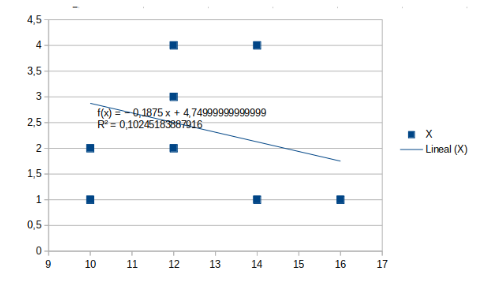
\includegraphics[width=\linewidth]{images/ejer_6_recta_X_Y.png}
        \end{subfigure}
        \begin{subfigure}[b]{0.45\linewidth}
        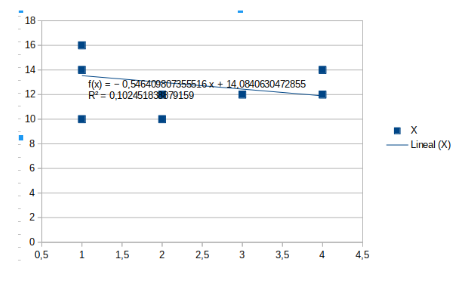
\includegraphics[width=\linewidth]{images/ejer_6_recta_Y_X.png}
        \end{subfigure}
    \end{figure}
    
    
Coeficiente de correlación lineal:
\[
    r = \pm\sqrt{r^2} = \frac{\sigma_{xy}}{\sigma_{x}\sigma_{y}} = \pm\sqrt{\frac{\sigma_{xy}^2}{\sigma_{x}^2\sigma_{y}^2}}
\]
\[
\sigma_{xy} < 0 \Longrightarrow r = -\sqrt{r^2} = \frac{-0,78}{\sqrt{4.16\cdot 1.428}} = -0,320
\]
El coeficiente de correlación lineal es negativo (por serlo la covarianza) y está más cerca del 0 que del -1, lo que indica una baja correlación lineal entre $X$ e $Y$.
Como se puede observar, la razón de correlación de nuestras rectas no supera a la recta de regresión de tipo 1 lo cual siempre se cumple.
\end{enumerate}

\end{ej}

\begin{ej}
Para cada una de las distribuciones:
\\
\\

\begin{center}
\begin{tabular}{c|ccc}[Distribución A]
	\(X/Y\) & 10 & 15 & 20 \\
	\hline
	1 & 0 & 2 & 0 \\
	2 & 1 & 0 & 0 \\
	3 & 0 & 0 & 3 \\
	4 & 0 & 1 & 0 \\
\end{tabular}  
\end{center}

\begin{center}
\begin{tabular}{c|ccc}[Distribución B]
	\(X/Y\) & 10 & 15 & 20 \\
	\hline
	1 & 0 & 2 & 0 \\
	2 & 1 & 0 & 0 \\
	3 & 0 & 0 & 3 \\
\end{tabular}
 \end{center}
 
 \begin{center}
\begin{tabular}{c|cccc}[Distribución C]
	\(X/Y\) & 10 & 15 & 20 & 25 \\
	\hline
	1 & 0 & 3 & 0 & 1 \\
	2 & 0 & 0 & 1 & 0 \\
	3 & 2 & 0 & 0 & 0 \\
\end{tabular}
\end{center}
\begin{enumerate}
    \item[a) ] ¿Dependen funcionalmente X de Y o Y de X? 
    \\
    \textbf{Dist. A:} Y depende funcionalmente de X, porque para cada valor de X solo existe un único valor de Y, en cambio X no depende funcionalmente de Y. \\
    \textbf{Dist. B:} X depende funcionalmente de Y y a la vez, Y depende funcionalmente de X. \\
    \textbf{Dist. C:} En este caso, X depende funcionalmente de Y pero Y no depende funcionalmente de X.
    \\
    Podemos observar que las distribuciones con tablas que no son cuadradas no pueden ser recíprocamente dependientes.
    \item[b) ] Calcular las curvas de regresión y comentar los resultados.
    La curva de regresión de tipo 1 de Y/X es la que viene dada por los puntos $(x_i, \bar{y}_i)$, la de X/Y es análoga, y viene dada por los puntos $(\bar{x}_j,y_j)$ con $i = 1, \dots , k$ y  $j = 1, \dots , p$.
   
        \textbf{Distribución A} \\
        Curva de regresión Y/X: \\
        $\bar{y}_1 = \frac{2 \cdot 15}{2} = 15$  $\bar{y}_2 = \frac{1 \cdot 10}{1} = 10$  $\bar{y}_3 = \frac{3 \cdot 20}{3} = 20$  $\bar{y}_4 = \frac{1 \cdot 15}{1} = 15$ \\
        Pasará por los puntos: $(1,15)$; $(2,10)$; $(3,20)$; $(4,15)$
        \begin{figure} [h]
        	\centering
    	    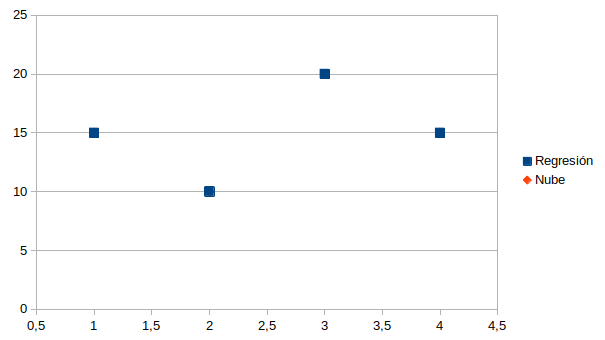
\includegraphics[scale=0.55]{images/ej7regxyA.png}
        \end{figure} \\
        Curva de regresión X/Y: \\
        $\bar{x}_1 = \frac{2 \cdot 1}{1} = 2$  $\bar{x}_2 = \frac{1 \cdot 2 + 1 \cdot 4}{3} = 2$  $\bar{x}_3 = \frac{3 \cdot 3}{3} = 3$ \\ 
        Pasará por los puntos: $(2,10)$; $(2,15)$; $(3,20)$ \\
        \begin{figure}[h]
        	\centering
    	    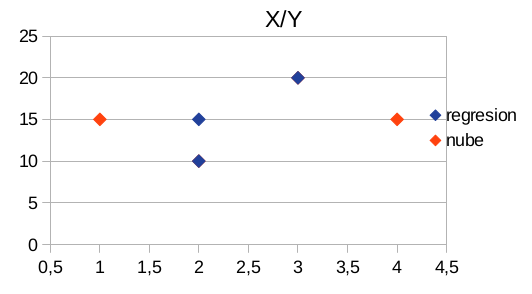
\includegraphics[scale=0.55]{images/ej7regyxA.png}
        \end{figure} 
        \textbf{Distribución B} \\
        Curva de regresión Y/X: \\
        $\bar{y}_1 = \frac{2 \cdot 15}{2} = 15$  $\bar{y}_2 = \frac{1 \cdot 10}{1} = 10$  $\bar{y}_3 = \frac{3 \cdot 20}{3} = 20$  \\
        Pasará por los puntos: $(1,15)$; $(2,10)$; $(3,20)$; \\
        \begin{figure}[h]
        	\centering
    	    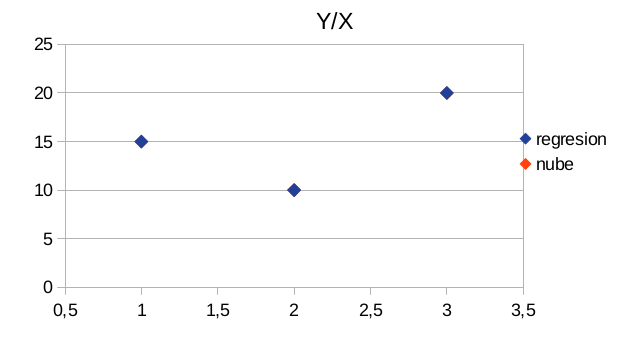
\includegraphics[scale=0.55]{images/ej7regyxB.png}
        \end{figure} \\
        Curva de regresión X/Y: \\
        $\bar{x}_1 = \frac{2 \cdot 1}{1} = 2$  $\bar{x}_2 = \frac{1 \cdot 2}{2} = 1$  $\bar{x}_3 = \frac{3 \cdot 3}{3} = 3$ \\ 
        Pasará por los puntos: $(2,10)$; $(1,15)$; $(3,20)$ \\
        \begin{figure}[h]
        	\centering
    	    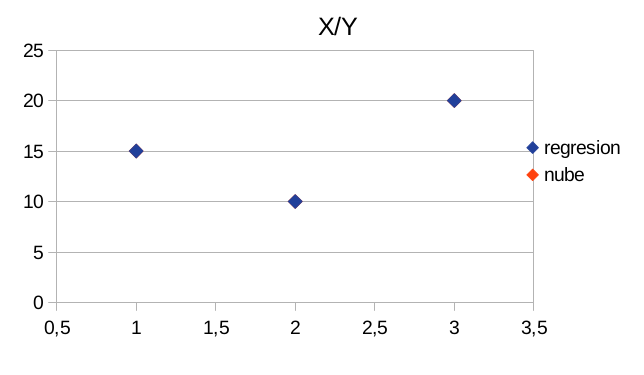
\includegraphics[scale=0.55]{images/ej7regxyB.png}
        \end{figure}
        \newpage
        \textbf{Distribución C} \\
        Curva de regresión Y/X: \\
        $\bar{y}_1 = \frac{3 \cdot 15 + 1 \cdot 25}{4} = 17.5$  $\bar{y}_2 = \frac{1 \cdot 20}{1} = 20$  $\bar{y}_3 = \frac{2 \cdot 10}{2} = 10$  \\
        Pasará por los puntos: $(1,17.5)$; $(2,20)$; $(3,10)$; \\
        \begin{figure}[h]
        	\centering
    	    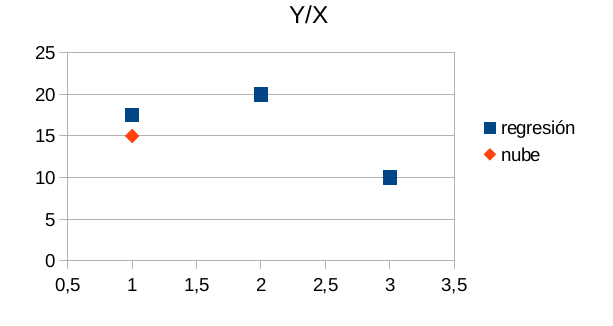
\includegraphics[scale=0.55]{images/ej7regyxC.png}
        \end{figure} \\
        Curva de regresión X/Y: \\
        $\bar{x}_1 = \frac{2 \cdot 3}{2} = 3$  $\bar{x}_2 = \frac{1 \cdot 3}{3} = 1$  $\bar{x}_3 = \frac{1 \cdot 2}{1} = 2$ $\bar{x}_4 = \frac{1 \cdot 1}{1} = 1$\\ 
        Pasará por los puntos: $(3,10)$; $(1,15)$; $(2,20)$ $(1,25)$\\
        \begin{figure}[h]
        	\centering
    	    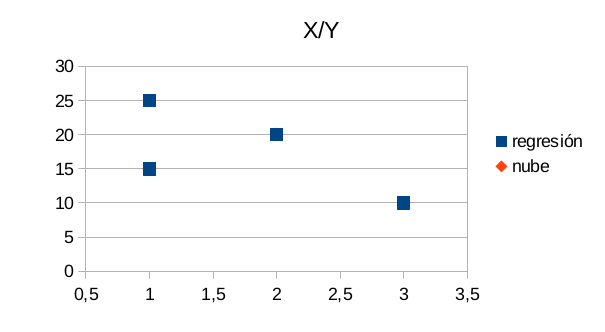
\includegraphics[scale=0.55]{images/ej7regxyC.png}
        \end{figure}
        \newpage
        
        
    Se pueden observar dos características de las curvas de regresión, en primer lugar, que en los casos en los que son funcionalmente dependientes , coinciden con la nube de puntos, además, cuando la dependencia es recíproca, la curva de regresión y la nube de puntos son iguales para X/Y, Y/X y entre ellas, como se ve en la distribución B.
    
\end{enumerate}
\end{ej}
 
\begin{ej}
De una muestra de 24 puestos de venta en un mercado de abastos se ha recogido información
sobre el número de balanzas (X) y el número de dependientes (Y ). Los resultados aparecen en
la siguiente tabla:

\begin{center}
\begin{tabular}{c|cccc}
	\(X/Y\) & 1 & 2 & 3 & 4 \\
	\hline
	1 & 1 & 2 & 0 & 0 \\
	2 & 1 & 2 & 3 & 1 \\
	3 & 0 & 1 & 2 & 6 \\
	4 & 0 & 0 & 2 & 3 \\
\end{tabular}
\end{center}

\begin{enumerate}[label=\alph*)]
\item Determinar las rectas de regresión.

Las rectas que se nos pide determinar son la recta de regresión lineal de \(Y\) sobre \(X\) y la recta de regresión lineal de \(X\) sobre \(Y\), las cuales vienen dadas por las siguientes expresiones respectivamente:
\[
	y - \overline{y}  =\frac{\sigma_{xy}}{\sigma_x^2} (x - \overline{x}) \Rightarrow y = \frac{\sigma_{xy}}{\sigma_x^2}x - \frac{\sigma_{xy}}{\sigma_x^2} \overline{x} + \overline{y}
\]

\[
	x - \overline{x}  =\frac{\sigma_{xy}}{\sigma_y^2} (y - \overline{y}) \Rightarrow x = \frac{\sigma_{xy}}{\sigma_y^2}y - \frac{\sigma_{xy}}{\sigma_y^2} \overline{y} + \overline{x}
\]

Por lo tanto, será necesario calcular las medias y varianzas marginales de cada carácter y la covarianza. Antes de desarrollar los cálculos de la tabla, vamos a especificar cómo calcularemos la covarianza. Como se vio en clase, $\sigma_{xy} = \mu_{11} = m_{11} -m_{10} m_{01}$, siendo $\mu_{rs}$ el momento conjunto central de órdenes r y s y $m_{rs}$ el momento conjunto respecto al origen de órdenes r y s. Recordemos que $m_{10} = \bar{x}$, $m_{01} = \bar{y}$ y $m_{11} = \sum_{i=1}^{k}\sum_{j=1}^{p}f_{ij}x_i y_j$. Procedamos a efectuar los cálculos pertinentes en la tabla:

\begin{center}
\begin{tabular}{c|cccc|ccc}
	\(X/Y\) & 1 & 2 & 3 & 4 & \(n_{i.}\) & \(n_{i.}x_i\) & \(n_{i.}x_i^2\) \\
	\hline
	1 & 1 & 2 & 0 & 0 & 3 & 3 & 3\\
	2 & 1 & 2 & 3 & 1 & 7 & 14 & 28\\
	3 & 0 & 1 & 2 & 6 & 9 & 27 & 81\\
	4 & 0 & 0 & 2 & 3 & 5 & 20 & 80\\
	\hline
	\(n_{.j}\) & 2 & 5 & 7 & 10 & 24 & 64 & 192 \\
	\(n_{.j} y_j\) & 2 & 10 & 21 & 40 & 73 \\
	\(n_{.j} y_j^2\) & 2 & 20 & 63 & 160 & 245 \\
	\(\sum_{i=1}^{k}n_{ij}x_i\) & 3 & 9 & 20 & 32 \\
\end{tabular}
\end{center}

\[
	m_{10} = \bar{x} = \frac{1}{n} \sum_{i=1}^{4} x_i n_{i.} = \frac{64}{24} = 2.667 \text{ balanzas}
\]

\[
    m_{01} = \bar{y} = \frac{1}{n} \sum_{j=1}^{4} n_{.j} y_j = \frac{73}{24} = 3.0417 \text{ dependientes}
\]

\[
	m_{11} = \sum_{i=1}^{4}\sum_{j=1}^{4}f_{ij}x_i y_j = \frac{1}{n}\sum_{j=1}^{4}\sum_{i=1}^{4}n_{ij}x_i y_j = \frac{1}{n}\sum_{j=1}^{4}y_j\sum_{i=1}^{4}n_{ij}x_i =
\]

\[
    = \frac{1 \cdot 2 + 2 \cdot 9 + 3 \cdot 20+4 \cdot 32}{24} = 8.708
\]

\[
    \sigma_{xy} = m_{11} -m_{10} m_{01} = 0.5958
\]

\[
    \sigma_{x}^{2} = \frac{1}{n} \sum_{i=1}^{4} n_{i.} x_i^2 - \overline{x}^2 = 0.8871  \text{ balanzas}^{2} \qquad \sigma_{y}^{2} = \frac{1}{n} \sum_{j=1}^{4} n_{.j} y_j^2 - \overline{y}^2 = 0.9564  \text{ dependientes}^{2}
\]

Ahora que tenemos todos los datos que necesitábamos, sustituimos sus valores en las expresiones de las rectas expuestas al principio del ejercicio:

\[
    y = \frac{\sigma_{xy}}{\sigma_x^2}x - \frac{\sigma_{xy}}{\sigma_x^2} \overline{x} + \overline{y} \Rightarrow y = 0.6716x+1.2505
\]

\[
    x = \frac{\sigma_{xy}}{\sigma_y^2}y - \frac{\sigma_{xy}}{\sigma_y^2} \overline{y} + \overline{x} \Rightarrow x = 0.623y+0.7721
\]

\newpage

\item ¿Es apropiado suponer que existe una relación lineal entre las variables?

Para ello, calcularemos el coeficiente de correlación de Pearson y a través de su interpretación podremos contestar esta pregunta:

\[
    r = \frac{\sigma_{xy}}{\sigma_x \sigma_y} = \frac{0.5958}{\sqrt{0.8871}\cdot\sqrt{0.9564}} = 0.6468
\]

En nuestro caso, $0 < r < 1$ $\Rightarrow$ Cuanto más próximo se encuentre $r$ de $1$, mejor dependencia lineal existirá entre el carácter $X$ y el carácter $Y$ en estudio. Sin embargo, 0.6468 es un valor que dista mucho de 1 como para poder considerar la relación lineal como la que mejor describe la relación del número de balanzas y de dependientes (se empezaría a considerar el coeficiente alto a partir de 0.85). Así, concluimos que no es apropiado suponer una relación lineal entre las variables.

\item Predecir, a partir de los resultados, el número de balanzas que puede esperarse en un puesto
con seis dependientes. ¿Es fiable esta predicción?

Para realizar la predicción haremos uso de la recta de regresión lineal de $X$ sobre $Y$, ya que se nos está proporcionando el número de dependientes:

\[
    x = 0.623 \cdot 6 + 0.7721 = 4.5101 \text{ balanzas (entre 4 y 5)}
\]

Por el apartado anterior, podemos afirmar que esta predicción no es fiable al estar basada en una relación lineal, pues esta no es la que mejor explica la relación entre las variables.
\end{enumerate}
\end{ej}


\begin{ej}
Se eligen 50 matrimonios al azar y se les pregunta la edad de ambos al contraer matrimonio. Los resultados se recogen en la siguiente tabla, en la que X denota la edad del hombre e Y la de la mujer:
\begin{center}
\begin{tabular}{c|ccccc}
	\(X/Y\) & (10,20] & (20,25] & (25,30] & (30,35] & (35,40] \\
	\hline
	(15,18] & 3 & 2 & 3 & 0 & 0 \\
	(18,21] & 0 & 4 & 2 & 2 & 0 \\
	(21,24] & 0 & 7 & 10 & 6 & 1\\
	(24,27] & 0 & 0 & 2 & 5 & 3\\
\end{tabular}
\end{center}
Estudiar la interdependencia lineal entre ambas variables.

\begin{center}
    \fbox{
    \begin{minipage}[h!]{1\linewidth}
    \begin{itemize}
        \item Población: los distintos matrimonios.
        \item Tamaño de la población: 50 matrimonios.
        \item Variable estadística: en este caso se presentan 2. \(X\) que es la del hombre al contraer matrimonio e \(Y\) que es la edad de la mujer en el mismo instante.
    \end{itemize}
    \end{minipage}
    }
\end{center}

Primero, se han de determinar las marcas de clase y crear la tabla con éstas:
\begin{center}
\begin{tabular}{c|ccccc|cccc}
	\(X/Y\) & 15 & 22.5 & 27.5 & 32.5 & 37.5 & $n_{i \cdot} $ & $c_i n_i$ & $c_i^2 n_i$ & $c_i \displaystyle\sum_{j=1}^5 n_{ij} c_j$\\
	\hline
	16.5 & 3 & 2 & 3 & 0 & 0 & 8 & 132 & 2178 & 2846.25 \\
	19.5 & 0 & 4 & 2 & 2 & 0 & 8 & 156 & 3042 & 4095 \\
	22.5 & 0 & 7 & 10 & 6 & 1 & 24 & 540 & 12150 & 14962.5 \\
	25.5 & 0 & 0 & 2 & 5 & 3 & 10 & 255 & 6502.5 & 8415 \\
	\hline
	$n_{\cdot j}$ & 3 & 13 & 17 & 13 & 4 & 50 &  &  & \vline 30318.75 \vline \\
	$c_j^2  n_{\cdot j}$ & 675 & 6581.25 & 12836.3 & 13731.3 & 5625 &  &  &  &  \\
\end{tabular}
\end{center}
$$\bar{x} = \dfrac{\displaystyle\sum_{j=1}^4 c_i \cdot n_{i \cdot}}{n} = 21.66 \text{ años hombre   } \bar{y} = \dfrac{\displaystyle\sum_{j=1}^5 c_j \cdot n_{\cdot j}}{n} = 27.55 \text{ años mujer}$$
\\
$$\sigma_x^2 = \frac{1}{n}\displaystyle\sum_{i=1}^4 n_{i \cdot} \cdot c_i^2 - \bar{x}^2 = 8.294 \implies \sigma_x = +\sqrt{\sigma_x^2} = 2.88 \text{ años hombre}$$
$$\sigma_y^2 = \frac{1}{n}\displaystyle\sum_{j=1}^5 n_{\cdot j} \cdot c_j^2 - \bar{y}^2 = 30.375 \implies \sigma_y = +\sqrt{\sigma_y^2} = 5.511 \text{ años mujer}$$
$$\sigma_{xy} = \frac{1}{n} \displaystyle \sum_{i=1}^4 \sum_{j=1}^5 n_{ij} \cdot c_i \cdot c_j -\bar{x}\bar{y} = 9.642$$
Ahora, si queremos determinar el grado de dependencia lineal debemos calcular el coeficiente de correlación lineal:
$$r = \dfrac{\sigma_{xy}}{\sigma_x \cdot \sigma_y} = 0.608$$
De este resultado se puede observar que la correlación es positiva y el grado de dependencia lineal es elevado.
\end{ej}

\bigskip

\begin{ej}
Calcular el coeficiente de correlación lineal de dos variables cuyas rectas de regresión son:
\[
	x + 4y = 1
\]
\[
	x + 5y = 2
\]

Como no nos indican cuál es la recta de regresión lineal \(Y/X\) y cúal es la \(X/Y\), supondremos que la pimera es la que explica la variable \(x\) en función de la variable \(y\) \((X/Y)\) y la segunda la que explica la variable \(y\) en función de la variable \(x\) y \((Y/X)\). \\

Se nos está pidiendo el coeficiente de correlación lienal \(r = \frac{\sigma_{xy}}{\sigma_x \sigma_y}\), y para hallarlo hemos de tener en cuenta la forma de dichas rectas para poder hallar \(\sigma_{xy}, \sigma_x, \text{ y } \sigma_y\):
\[
	x + 4y = 1 \Rightarrow x = 1 - 4y \Rightarrow x = \frac{\sigma_{xy}}{\sigma_y^2}y + \overline{x} - \frac{\sigma_{xy}}{\sigma_y^2} \overline{y}
\]
\[
	x +5y = 2 \Rightarrow y = - \frac{1}{5}x + \frac{2}{5} \Rightarrow y = \frac{\sigma_{xy}}{\sigma_x^2}x -\frac{\sigma_{xy}}{\sigma_x^2} \overline{x} + \overline{y}
\]

Por otro lado:
\[
	r^2 = \frac{\sigma_{xy}}{\sigma_y^2} \cdot \frac{\sigma_{xy}}{\sigma_x^2} = (-4) \cdot (-\frac{1}{5}) = \frac{4}{5} \Rightarrow r = -\sqrt{r^2} = -0.89443
\]
Es necesario mencionar que tomamos el valor negativo de la raíz pues sabemos que la covarianza es negativa. \\

Como \(r \in [-1, 0]\), sabemos que es un resultado lógico. Veamos qué hubiese ocurrido si las rectas las hubieramos tomado del revés:
\[
	x + 4y = 1 \Rightarrow y = - \frac{1}{4}x + \frac{1}{4} \Rightarrow y = \frac{\sigma_{xy}}{\sigma_x^2}x + \overline{y} - \frac{\sigma_{xy}}{\sigma_x^2} \overline{x}
\]
\[
	x + 5y = 2 \Rightarrow x = -5y +2 \Rightarrow x = \frac{\sigma_{xy}}{\sigma_y^2}y + \overline{x} - \frac{\sigma_{xy}}{\sigma_y^2} \overline{y}
\]

Actuamos igual que antes:
\[
	r^2 = \frac{\sigma_{xy}}{\sigma_x^2} \cdot \frac{\sigma_{xy}}{\sigma_y^2} = (-\frac{1}{4}) \cdot (-5) = \frac{5}{4} \Rightarrow r = -\sqrt{r^2} = -1.11803
\]

Observamos que \(r < -1\). Esto no tiene ningún tipo de sentido, por lo que la interpretación correcta era la anterior.
\end{ej}

\vspace{2mm}

\begin{ej}
Consideremos una distribución bidimensional en la que la recta de regresión de $Y$ sobre $X$ es $y=5x-20$, y $\sum y_j^2n_{.j} = 3240$. Supongamos, además, que la distribución marginal de $X$ es:

\begin{center}
\begin{tabular}{c|cccc}
    $x_i$ & 3 & 5 & 8 & 9 \\
    \hline
    $n_{i.}$ & 5 & 1 & 2 & 1 
\end{tabular}
\end{center}

Determinar la recta de regresión de $X$ sobre $Y$ , y la bondad de los ajustes lineales.

\begin{center}
\begin{tabular}{c|cccc|c}
    $x_i$ & 3 & 5 & 8 & 9 & 25 \\
    \hline
    $n_{i.}$ & 5 & 1 & 2 & 1 & 9\\
    \hline
    $x_in_{i.}$ & 15 &  5 & 16 & 9 & 45 \\
    \hline
    $x_i^2n_{i.}$ & 45 & 25 & 128 & 81 & 279 \\
\end{tabular}
\end{center}

\[
\overline{x} = \frac{1}{n}\sum_{i=1}^4x_in_{i.}= \frac{1}{\sum^4_{i=1}n_{i.}}\sum_{i=1}^4x_in_{i.}=\frac{45}{9} = 5
\]
\[
\sigma_x^2 = \frac{1}{n}\sum_{i=1}^4n_{i.}x_i^2 - \overline{x}^2 = \frac{279}{9} -25 = 6
\]
\[
\frac{\sigma_{xy}}{\sigma_x^2}=5 \Longrightarrow \sigma_{xy} = 5 \cdot\sigma_x^2= 5\cdot 6 = 30
\]
\[
\overline{y}=5\overline{x} -20 = 25-20 = 5
\]
\[
\sigma_y^2 = \frac{1}{n}\sum_{j=1}^4n_{.j}y_j^2 -\overline{y}^2 = \frac{3240}{9}-5^2 = 335
\]
Recta de regresión de $X$ sobre $Y$:
\[
x - \overline{x} = \frac{\sigma_{xy}}{\sigma_{y}^2} \cdot (y - \overline{y}) \Longrightarrow x=\frac{\sigma_{xy}}{\sigma_y^2}y-\frac{\sigma_{xy}}{\sigma_y^2}\overline{y}+\overline{x}= \frac{30}{335}y-\frac{30}{335}\cdot 5 + 5 \Longrightarrow x = 0.090y + 4.552
\]
Coeficiente de determinación lineal
\[
\eta_{Y/X}^{2} = \frac{\sigma_{xy}^2}{\sigma_y^2\sigma_x^2} = \frac{30^2}{6\cdot 335} = 0.448 \Longrightarrow \text{explican el 44.80\% de los casos}
\]
Las rectas de regresión explican menos del 50\% de los casos, lego podemos conluir que no se trata de un buen ajuste.

\end{ej}

\begin{ej}
De las estadísticas de ”Tiempos de vuelo y consumos de combustible ”de una compañía aérea, se
han obtenido datos relativos a 24 trayectos distintos realizados por el avión DC-9. A partir de
estos datos se han obtenido las siguientes medidas:

\[
    \sum_{j=1}^{p}n_{.j}y_j = 219.719 \qquad \sum_{j=1}^{p}n_{.j}y_{j}^{2} = 2396.504 \qquad \sum_{i=1}^{k}\sum_{j=1}^{p}n_{ij}x_i y_j = 349.486
\]

\[
    \sum_{i=1}^{k}n_{i.}x_i = 31.470 \qquad \sum_{i=1}^{k}n_{i.}x_{i}^{2} = 51.075 \qquad \sum_{i=1}^{k}\sum_{j=1}^{p}n_{ij}x_{i}^{2} y_j = 633.993
\]

\[
    \sum_{i=1}^{k}\sum_{j=1}^{p}n_{ij}x_{i}^{4} = 182.977 \qquad \sum_{i=1}^{k}\sum_{j=1}^{p}n_{ij}x_{i}^{3} = 93.6
\]

La variable Y expresa el consumo total de combustible, en miles de libras, correspondiente a
un vuelo de duración X (el tiempo se expresa en horas, y se utilizan como unidades de orden
inferior fracciones decimales de la hora).

\begin{enumerate}[label=\alph*)]
\item Ajustar un modelo del tipo $Y = aX +b$. ¿Qué consumo total se estimaría para un programa
de vuelos compuesto de 100 vuelos de media hora, 200 de una hora y 100 de dos horas? ¿Es
fiable esta estimación?

Hemos de calcular la expresión de la recta de regresión lineal de Y sobre X, la cual es de la forma:

\[
    y - \overline{y}  =\frac{\sigma_{xy}}{\sigma_x^2} (x - \overline{x}) \Rightarrow y = \frac{\sigma_{xy}}{\sigma_x^2}x - \frac{\sigma_{xy}}{\sigma_x^2} \overline{x} + \overline{y}
\]

Procederemos como en ejercicios anteriores calculando las medias marginales $m_{10} = \bar{x}$ y $m_{11} = \bar{y}$, la varianza del carácter X que es $\sigma_{x}^{2} = \frac{1}{n} \sum_{i=1}^{k} n_{i.} x_i^2 - \overline{x}^{2}$ y la covarianza, que es $\sigma_{xy} = \mu_{11} = m_{11} - m_{10}m_{01} = \frac{1}{n}\sum_{i=1}^{k}\sum_{j=1}^{p}n_{ij}x_i y_j - \bar{x}\bar{y}$. En este caso no se requiere hacer tabla, ya que se nos han proporcionado todos los datos necesarios para calcular lo que necesitamos:

\[
    m_{10} = \bar{x} = \frac{1}{n} \sum_{i=1}^{k} x_i n_{i.} = \frac{31.470}{24} = 1.3113 \text{ horas de vuelo} \qquad
\]

\[
    m_{01} = \bar{y} = \frac{1}{n} \sum_{j=1}^{p} n_{.j} y_j = \frac{2396.504}{24} = 9.155 \text{ miles de libras de combustible}
\]


\[
    m_{11} = \frac{1}{n}\sum_{i=1}^{k}\sum_{j=1}^{p}n_{ij}x_i y_j = \frac{349.486}{24} = 14.5619 \qquad \mu_{11} = \sigma_{xy} = m_{11} - m_{10}m_{01} = 2.557
\]

\[
    \sigma_{x}^{2} = \frac{1}{n} \sum_{i=1}^{k} n_{i.} x_i^2 - \overline{x}^2 = \frac{51.075}{24}-1.3113^{2} = 0.4086 \text{ horas de vuelo}^{2}
\]

\[
    \sigma_{y}^{2} = \frac{1}{n} \sum_{j=1}^{p} n_{.j} y_j^2 - \overline{y}^2 = \frac{2396.504}{24}-9.155^{2} = 16.0403 \text{ miles de libras de combustible}^{2}
\]
Y sustituimos los valores calculados en la expresión de la recta:

\[
    y = \frac{\sigma_{xy}}{\sigma_x^2}x - \frac{\sigma_{xy}}{\sigma_x^2} \overline{x} + \overline{y} \Rightarrow y = 6.258x+0.9489
\]

Haciendo uso de esta recta, podemos estimar el consumo total de combustible tras 100 vuelos de media hora, 200 de una hora y 100 de dos horas respectivamente: 

\[
    y = 6.258 \cdot 0.5 \cdot 100 + 0.9489 = 4.0779 \text{ miles de libras de combustible}
\]

\[
    y = 6.258 \cdot 1 + 0.9489 = 7.2069 \text{ miles de libras de combustible}
\]

\[
    y = 6.258 \cdot 2 + 0.9489 = 13.4649 \text{ miles de libras de combustible}
\]

\[
    \text{Combustible total} = 4.0779 \cdot 100 + 7.2069 \cdot 200 + 13.4649 \cdot 100 = 3195.66 \text{ miles de libras}
\]
 
Para saber si esta estimación es fiable, calcularemos el coeficiente de correlación de Pearson y lo interpretaremos:

\[
    r = \frac{\sigma_{xy}}{\sigma_x \sigma_y} = \frac{2.557}{\sqrt{0.4086}\cdot\sqrt{16.0403}} = 0.9988
\]

En nuestro caso, $0 < r < 1$ $\Rightarrow$ Cuanto más próximo se encuentre $r$ de $1$, mejor dependencia lineal existirá entre el carácter $X$ y el carácter $Y$ en estudio. Como $r$ es prácticamente 1, l relación lineal explica de forma óptima la relación entre las variables y podemos afirmar que las estimaciones hechas son fiables.

\item Ajustar un modelo del tipo $Y = a + bX + cX^2$ . ¿Qué consumo total se estimaría para el
mismo programa de vuelos del apartado a)?

Para poder hallar los coeficientes $a$, $b$ y $c$ y ajustar al modelo pedido necesitamos minimizar la siguiente función:

\[
    \psi(a,b,c) = \sum_{i=1}^{k}\sum_{j=1}^{p}f_{ij}(y_j-a-bx_i-cx_{i}^{2})^2
\]

\[
    \psi(a,b,c) = \sum_{i=1}^{k}\sum_{j=1}^{p}f_{ij}(y_{j}^2-2ay_j-2bx_i y_j -2cx_{i}^{2}y_j+a^2+2abx_i+2acx_{i}^{2}+b^2 x_{i}^{2}+2bcx_{i}^{3}+c^2 x_{i}^{4})
\]

Ahora hallaremos las derivadas parciales de dicha función y las igualaremos a 0, obteniendo así un SEL compatible determinado del cual despejaremos los valores de $a$, $b$ y $c$:

\[
    \frac{\partial\psi(a,b,c)}{\partial a} = -2\sum_{i=1}^{k}\sum_{j=1}^{p}f_{ij}y_j + 2a + 2b\sum_{i=1}^{k}\sum_{j=1}^{p}f_{ij}x_i + 2c\sum_{i=1}^{k}\sum_{j=1}^{p}f_{ij}x_{i}^{2} = 
\]

\[
    = -2m_{01}+2a+2bm_{10}+2cm_{20}
\]

Hallamos $m_{20}$, que no habíamos calculado:

\[
    m_{20} = \frac{1}{n}\sum_{i=1}^{k}\sum_{j=1}^{p}n_{ij}x_{i}^{2} = \frac{51.075}{24} = 2.1281
\]

Y sustituimos $m_{01}$, $m_{10}$ y $m_{20}$ en la expresión anterior igualándola a 0 para obtener la primera ecuación del sistema:

\[
    -2m_{01}+2a+2bm_{10}+2cm_{20} = 0 \Rightarrow a+1.3113b+2.1281c=9.155
\]

Repetimos el proceso con las derivadas parciales en función de $b$ y de $c$:

\[
    \frac{\partial\psi(a,b,c)}{\partial b} = -2\sum_{i=1}^{k}\sum_{j=1}^{p}f_{ij}x_i y_j + 2a\sum_{i=1}^{k}\sum_{j=1}^{p}f_{ij}x_i + 2b\sum_{i=1}^{k}\sum_{j=1}^{p}f_{ij}x_{i}^{2}+ 2c\sum_{i=1}^{k}\sum_{j=1}^{p}f_{ij}x_{i}^{3} = 
\]

\[
    = -2m_{11}+2am_{10}+2bm_{20}+2cm_{30}
\]

Calculamos $m_{30}$:

\[
    m_{30} = \frac{1}{n}\sum_{i=1}^{k}\sum_{j=1}^{p}n_{ij}x_{i}^{3} = \frac{93.6}{24} = 3.9
\]

Y sustituimos en la expresión igualándola a 0 para obtener la segunda ecuación del sistema:

\[
    -2m_{11}+2am_{10}+2bm_{20}+2cm_{30} = 0 \Rightarrow 1.3113a+2.1281b+3.9c=14.5619
\]

\[
    \frac{\partial\psi(a,b,c)}{\partial c} = -2\sum_{i=1}^{k}\sum_{j=1}^{p}f_{ij}x_{i}^{2} y_j + 2a\sum_{i=1}^{k}\sum_{j=1}^{p}f_{ij}x_{i}^{2} + 2b\sum_{i=1}^{k}\sum_{j=1}^{p}f_{ij}x_{i}^{3}+ 2c\sum_{i=1}^{k}\sum_{j=1}^{p}f_{ij}x_{i}^{4} = 
\]

\[
   = -2m_{21}+2am_{20}+2bm_{30}+2cm_{40}
\]

Calculamos $m_{21}$ y $m_{40}$:

\[
    m_{21} = \frac{1}{n}\sum_{i=1}^{k}\sum_{j=1}^{p}n_{ij}x_{i}^{2} = \frac{633.993}{24} = 26.4139 \qquad m_{40} = \frac{1}{n}\sum_{i=1}^{k}\sum_{j=1}^{p}n_{ij}x_{i}^{4} = \frac{182.977}{24} = 7.6240
\]

Y sustituimos en la expresión anterior igualándola a 0 para obtener la última ecuación del sistema:

\[
    = -2m_{21}+2am_{20}+2bm_{30}+2cm_{40} \Rightarrow 2.1281a+3.9b+7.624c = 26.4139
\]

Y resolvemos el sistema resultante:
\[
\left.
\begin{array}{rcl}
     a+1.3113b+2.1281c&=&9.155
  \\ 1.3113a+2.1281b+3.9c&=&14.5619
  \\ 2.1281a+3.9b+7.624c &=& 26.4139
\end{array}
\right\}
\]

La solución del sistema es: $a=0.7491$, $b=6.6368$ y $c=-0.1395$ y por lo tanto la parábola del modelo que se nos pedía es de la forma $y=0.7491+6.6368x-0.1395x^2$. Realicemos las estimaciones que se nos pedían el apartado a) pero con el nuevo modelo:

\[
    y = 0.7491+6.6368 \cdot 0.5 -0.1395 \cdot 0.5^2 = 4.0326 \text{ miles de libras de combustible}
\]

\[
    y = 0.7491+6.6368 \cdot 1 -0.1395 \cdot 1^2 =  7.2464\text{ miles de libras de combustible}
\]

\[
    y = 0.7491+6.6368 \cdot 2 -0.1395 \cdot 2^2 =  13.4647 \text{ miles de libras de combustible}
\]

\[
    \text{Combustible total} = 4.0326 \cdot 100 + 7.2464 \cdot 200 + 13.4647 \cdot 100 = 3199.01 \text{ miles de libras}
\]

\item ¿Cuál de los dos modelos se ajusta mejor? Razonar la respuesta.

Al observar el segundo modelo, podemos notar que la ecuación del modelo es prácticamente idéntica a la del primer modelo exceptuando el término $-0.1395x^2$. De hecho, en las estimaciones realizadas, ambos modelos nos dan un valor muy parecido (casi 3200). Este modelo es más fino ya que el término $-0.1395x^2$ está añadiendo información a la recta del modelo del apartado a), es decir, no se pierde la información que había en el modelo 1. En conclusión, la razón de correlación de la parábola siempre será mayor o igual que la de la recta.

\end{enumerate}
\end{ej}

\begin{ej}
La curva de Engel, que expresa el gasto en un determinado bien en función de la renta, adopta en ocasiones la forma de una hipérbola equilátera. Ajustar dicha curva a los siguientes datos, en los que \(X\) denota la renta en miles de euros e \(Y\) el gasto en euros. Cuantificar la bondad del ajuste:

\begin{center}
    \fbox{
    \begin{minipage}[h!]{1\linewidth}
    \begin{itemize}
        \item Población: las distintas rentas.
        \item Tamaño de la población: 4 rentas.
        \item Variable estadística: en este caso se presentan 2. \(X\) que es el total de la renta e \(Y\) que es el gasto en un determinado bien (en miles de euros).
    \end{itemize}
    \end{minipage}
    }
\end{center}
\begin{center}
\begin{tabular}{c|cccc}
	\(X\) 10 & 12.5 & 20 & 25 \\
	\hline
	\(Y\) 50 & 90 & 160 & 180 \\
\end{tabular}
\end{center}

Por lo visto en teoría en clase, la hipérbola equilátera es un modelo de regresión dado por la función
\[
	y = f(x) = a \frac{1}{x} + b
\]

Para poder terminar \(a\) y \(b\), hemos de linealizar realizando la siguiente transformación: \(z = \frac{1}{x}\). Esto nos permite expresar la anterior función de la siguiente forma:
\[
	y = az + b
\]

Y ya, simplemente hemos de hallar \(a\) y \(b\) como si de una recta de regresión lineal se tratase, por lo que:
\[
	a = \frac{\sigma_{zy}}{\sigma_z^2} \qquad b = \overline{y} - a \overline{z} \Rightarrow b = \overline{y} - \frac{\sigma_{zy}}{\sigma_z^2}
\]

Efectuamos los cálculos:
\[
	\overline{z} = \frac{1}{n} \sum_{i=1}^{4} n_{i.} z_i = \frac{\frac{1}{10}+\frac{1}{12.5}+\frac{1}{20}+\frac{1}{25}}{4} = 0.0675 \text{ miles de euros}^{-1}
\]
\[
	\overline{y} = \frac{1}{n} \sum_{j=1}^{4} n_{.j} y_j = \frac{50 + 90 + 160 + 180}{4} = 120 \text{ euros}
\]
\[
	\sigma_z^2 = \frac{1}{n} \sum_{i=1}^{4} n_{i.} z_i^2 - \overline{z}^2 = \frac{0.0205}{4} - 0.0675^2 = 0.00056875 \text{ miles de euros}^{-2}
\]

\[
	\sigma_{zy} = m_{11} - m_{10} m_{01} 
\]
\[
	m_{11} = \frac{1}{n} \sum_{i=1}^{k} \sum_{j=1}^{p} n_{i.} z_i y_j = \frac{5 + \frac{36}{5} + 8 + \frac{36}{5}}{4} = 6.85
\]
\[
	\sigma_{zy} = 6.85 - 120 \cdot 0.0675 = -1.25
\]

Así, ya podemos calcular los parámetros \(a\) y \(b\):
\[
	a = \frac{-1.25}{0.00056875} = -2197.8
\]
\[
	b = 120 + 2197.8 \cdot 0.0675 = 268.35
\]

Por lo tanto la recta de regresión que buscamos era:
\[
	y = -2197.8z + 268.35
\]

Y deshaciendo el cambio auxiliar, la hipérbola equilátera será de la forma:
\[
	y = - \frac{2197.8}{x} + 268.35
\] \\

Para poder determinar la bondad del ajuste lineal, necesitamos interpretar el coeficiente de determinación, que tiene la siguiente forma:
\[
	\eta_{Y/X}^2 = 1 - \frac{\sigma_{ey}^2}{\sigma_y^2} \rightarrow \text{ varianza residual}
\]

Para poder calcularlo nos falta el valor de la varianza residual y de la varianza de \(y\):
\[
	\sigma_{ey}^2 = \frac{1}{n} \sum_{i=1}^{k} \sum_{j=1}^{p} (y_j - f(x_i))^2 f_{ij} = \frac{1}{n} \sum_{i=1}^{k} \sum_{j=1}^{p} n_{ij} (y_j - (a \frac{1}{x_i} + b)^2 = 2.64563
\]
\[
	\sigma_y^2 = \frac{1}{n} \sum_{j=1}^{p} n_{.j} y_j^2 - \overline{y}^2 = \frac{2500+8100+25600+32400}{4} - 120^2 = 2750 \text{ euros}^2
\]

Así:
\[
	\eta_{Y/X}^2 = 1 - \frac{2.64563}{2750} = 0.9990379
\]

Sabemos siempre que \(0 \leq \eta_{X/Y}^2 \leq 1\). Cuanto más próximo esté este valor a 1, mejor correlación existirá entre las variables según la función de regresión ajustada. Como en este caso es casi 1, podemos afirmar que hay una correlación prácticamente perfecta y concluimos que el ajuste es muy bueno.
\end{ej}
\begin{ej}
Se dispone de la siguiente información referente al gasto en espectáculos (Y, en euros) y la rentadisponible mensual (X, en cientos de euros) de 6 familias: \\ \\
\centering
\begin{tabular}{c|cccccc}
    Y & 30 & 50 & 70 & 80 & 120 & 140\\ \hline
    X & 9 & 10 & 12 & 15 & 22 & 32
\end{tabular} \\
Explicar el comportamiento de Y por X mediante: \\
\begin{enumerate}
    \item[a) ] Relación lineal. \\
    Para esto, debemos calcular la recta de regresión, que viene dada por:
    $$y = \bar{y} + \frac{\sigma_{xy}}{\sigma_x^2}x - \frac{\sigma_{xy}}{\sigma_x^2}\bar{x}$$
    Para realizar la recta, usaré una tabla para ir almacenando los cálculos: \\
    \begin{tabular}{c|cccccc|cccc}
    X/Y & 30 & 50 & 70 & 80 & 120 & 140 & $n_{i \cdot}$ & $n_{i \cdot} x_i$ &  $n_{i \cdot} x_i^2$ & $x_i \displaystyle \sum_{i = 1}^6 n_{ij} y_j$\\
    \hline
    9 & 1 & 0 & 0 & 0 & 0 & 0 & 1 & 9 & 81 & 270 \\
    10 & 0 & 1 & 0 & 0 & 0 & 0 & 1 & 10 & 100 & 500 \\
    12 & 0 & 0 & 1 & 0 & 0 & 0 & 1 & 12& 144 & 840 \\
    15 & 0 & 0 & 0 & 1 & 0 & 0 & 1 & 15 & 225 & 1200 \\
    22 & 0 & 0 & 0 & 0 & 1 & 0 & 1 & 22 & 484 & 2640 \\
    32 & 0 & 0 & 0 & 0 & 0 & 1 & 1 & 32 & 1024 & 4480 \\
    \hline
    $n_{\cdot j}$ & 1 & 1 & 1 & 1 & 1 & 1 & 6 & & & \vline 9930 \vline \\
    $n_{\cdot j} y_j$ & 30 & 50 & 70 & 80 & 120 & 140 & & & &\\
    $n_{\cdot j} y_j^2$ & 900 & 2500 & 4900 & 6400 & 14400 & 19600
    \end{tabular}
    
    $$\bar{x} = \frac{\displaystyle\sum_{i=1}^6 x_i \cdot n_{i \cdot}}{n} = 16.667 \text{ cientos de euros} \ \bar{y} = \frac{\displaystyle\sum_{j=1}^6 y_j \cdot n_{\cdot j}}{n} = 81.667 \text{ euros}$$
    $$\sigma_x^2 = \frac{1}{n} \displaystyle \sum_{i = 1}^6 n_{i \cdot} \cdot x_i^2 - \bar{x}^2 = 65.221 \text{ cientos de euro} s^2$$
    $$\sigma_y^2 = \frac{1}{n} \displaystyle \sum_{j = 1}^6 n_{\cdot j} \cdot y_j^2 - \bar{y}^2 = 1447.217 \text{ euro} s^2$$
    $$\sigma_{xy} = \frac{1}{n}   \displaystyle \sum_{i = 1}^6 \sum_{j=1}^6 n_{ij} \cdot x_i \cdot y_i - \bar{x} \bar{y} = 293.884$$
    \\
    Sustituyendo en la expresión al principio del apartado, $y = 4.506x + 6.567$.
    \\
    Para ver cómo de bueno es el ajuste, calcularemos el coeficiente de determinación lineal:
    $$ r^2 = \dfrac{\sigma_{xy}^2}{\sigma_x^2 \sigma_y^2} = 0.915$$
    \item[b) ] Hipérbola equilátera.
    \\
    Es de la forma : $y = \frac{a}{x} + b$, si $z = \frac{1}{x}$ entonces buscaremos $y = az + b$. \\
    
    \begin{tabular}{c|cccccc}
         Y & 30 & 50 & 70 & 80 & 120 & 140 \\ \hline
         Z & 0.111 & 0.1 & 0.083 & 0.067 & 0.046 & 0.031
    \end{tabular} \\
    $$\bar{z} = \dfrac{\displaystyle \sum_{i = 1}^6 z_i \cdot n_{i \cdot}}{n} = 0.073 $$
    $$\sigma_z^2 = \frac{1}{n} \displaystyle \sum_{i = 1}^6 n_{i \cdot} \cdot z_i^2 - \bar{z}^2 = 0.0008 $$
    $$\sigma_{zy} = \frac{1}{n}   \displaystyle \sum_{i = 1}^6 \sum_{j=1}^6 n_{ij} \cdot z_i \cdot y_i - \bar{z} \bar{y} = -1.069$$
    $$y = \bar{y} + \frac{\sigma_{zy}}{\sigma_z^2}z - \frac{\sigma_{zy}}{\sigma_z^2}\bar{z}$$
    $$y = -1333.712z + 179.25$$
    Sustituyendo la z: 
    $$y = -\frac{1333.712}{x} + 179.2501$$
    \\
    Al igual que en el apartado anterior, debemos calcular la razón de correlación para ver como de bueno es el ajuste:
    \\
    $$\eta_{Y/X}^2 = \frac{\sigma_{ey}^2}{\sigma_y^2}.$$
    $$\sigma_{ey}^2 = \frac{1}{n} \displaystyle\sum_{i = 1}^6 \sum_{j = 1}^6 n_{ij}(f(x_i) - \bar{y})^2$$
    $$f(9) = 31.0598$$
    $$f(10) = 45.8789$$
    $$f(12) = 68.1074$$
    $$f(15) = 90.3359$$
    $$f(22) = 118.6268$$
    $$f(32) = 137.5716$$
    $$\displaystyle\sum_{i=1}^6 \sum_{j=1}^6 n_{ij}(f(x_i) - \bar{y})^2 = 2561.058 + 1280.767 + 183.855 + 75.153 + 1366.049 + 3125.337 = 8592.241$$
    $$\sigma_{ey}^2 = \frac{1}{n} \displaystyle\sum_{i = 1}^6 \sum_{j=1}^6 n_{ij}(f(x_i) - \bar{y})^2 = 1432.04$$
    $$\eta_{Y/X}^2 = \dfrac{\sigma_{ey}^2}{\sigma_y^2} = 0.99$$
    \item[c) ] Curva potencial
    \\
    Es de la forma $y = bx^a$. Para lo que haré:
    $$log \ y = log \ bx^a \iff log \ y = log \ b + alog \ x$$
    $$y' = az + b' \text{ con } y' = log \ y \ \ b' = log \ b \  \ z' = log \ x $$
    \\
    \begin{tabular}{c|cccccc}
         Y' & 3.401 & 3.912 & 4.249 & 4.382 & 4.788 & 4.942 \\ \hline
         Z & 2.197 & 2.303 & 2.485 & 2.708 & 3.091 & 3.466
    \end{tabular}
    \\
    $$\bar{z} = \dfrac{\displaystyle \sum_{i = 1}^6 z_i \cdot n_{i \cdot}}{n} = 2.708 $$
    $$\bar{y'} = \dfrac{\displaystyle \sum_{j = 1}^6 y_j \cdot n_{\cdot j}}{n} = 4.273 $$
    $$\sigma_z^2 = \frac{1}{n} \displaystyle \sum_{i = 1}^6 n_{i \cdot} \cdot z_i^2 - \bar{z}^2 = 0.199$$
    $$\sigma_{zy'} = \frac{1}{n}   \displaystyle \sum_{i = 1}^6 \sum_{j=1}^6 n_{ij} \cdot z_i \cdot y'_i - \bar{z} \bar{y'} = 0.217$$
    
    $$y = \bar{y} + \frac{\sigma_{zy'}}{\sigma_z^2}\cdot z - \frac{\sigma_{zy'}}{\sigma_x^2}\cdot \bar{z}$$
    
    $$y = 1.0884z + 1.331$$
    $$b = e^{b'} = 3.785$$
    $$y = 3.785x^{1.088}$$
    \\
    Con una razón de correlación:
    $$\eta_{Y/X}^2 = 1 - \frac{\sigma_{ey}^2}{\sigma_y^2}$$
    $$f(9) = 41.368$$
    $$f(10) = 46.394$$
    $$f(12) = 56.778$$
    $$f(15) = 72.131$$
    $$f(22) = 109.436$$
    $$f(32) = 164.334$$
    $$\sigma_{ey}^2 = \frac{1}{n} \displaystyle \sum_{i = 1}^6 \sum_{j = 1}^6 n_{ij} (y_j - f(x_i))^2 = 183.019$$
    $$\eta_{Y/X}^2 = 1 - \frac{\sigma_{ey}^2}{\sigma_y^2} = 0.874$$
    \item[d) ] Curva exponencial \\
    $$y = ba^x \iff log \ y = log \ b + xlog \ a$$
    $$y' = b' + xa' \text{ con } y' = log \ y b' = log \ b a' = log \ a$$
    \\ 
    \begin{tabular}{c|cccccc}
        Y' & 3.401 & 3.912 & 4.249 & 4.382 & 4.788 & 4.942\\ \hline
        X  & 9 & 10 & 12 & 15 & 22 & 32 
    \end{tabular} \\
    Del primer apartado sabemos que:
    $$\bar{x} = 16.667 \ \ \sigma_x^2 = 65.221$$
    $$\sigma_{xy'} = \frac{1}{n} \displaystyle \sum_{i = 1}^6 \sum_{j = 1}^6 n_{ij} \cdot x_i \cdot y'_j - \bar{x} \cdot \bar{y'} = 3.67$$
    $$y' = 0.056x + 3.341$$
    $$a = e^{a'} = 1.058 \ \ b = e^{b'} = 28.247$$
    $$y = 28.247 \cdot 1.058^x$$
     Con una razón de correlación:
    $$\eta_{Y/X}^2 = 1 - \frac{\sigma_{ey}^2}{\sigma_y^2}$$
    $$f(9) = 46.879$$
    $$f(10) = 49.593$$
    $$f(12) = 55.503$$
    $$f(15) = 65.712$$
    $$f(22) = 97.445$$
    $$f(32) = 171.083$$
    $$\sigma_{ey}^2 = \frac{1}{n} \displaystyle \sum_{i = 1}^6 \sum_{j = 1}^6 n_{ij} (y_j - f(x_i))^2 = 362.372$$
    $$\eta_{Y/X}^2 = 1 - \frac{\sigma_{ey}^2}{\sigma_y^2} = 0.75$$
    \
    \
    De aquí observamos que el ajuste más adecuado es el del apartado b, la hipérbola equilátera, ya que su razón de correlación se acerca más a 1 que las demás y por tanto es la que mejor se ajusta a la nube de puntos.
    \end{enumerate}
\end{ej}
\end{document}